\documentclass[10pt]{beamer}
\usetheme[
%%% option passed to the outer theme
%    progressstyle=fixedCircCnt,   % fixedCircCnt, movingCircCnt (moving is deault)
  ]{Feather}
  
% If you want to change the colors of the various elements in the theme, edit and uncomment the following lines

% Change the bar colors:
%\setbeamercolor{Feather}{fg=red!20,bg=red}

% Change the color of the structural elements:
%\setbeamercolor{structure}{fg=red}

% Change the frame title text color:
%\setbeamercolor{frametitle}{fg=blue}

% Change the normal text color background:
%\setbeamercolor{normal text}{fg=black,bg=gray!10}

%-------------------------------------------------------
% INCLUDE PACKAGES
%-------------------------------------------------------

\usepackage[utf8]{inputenc}
\usepackage[english]{babel}
\usepackage[T1]{fontenc}
\usepackage{helvet}

%-------------------------------------------------------
% DEFFINING AND REDEFINING COMMANDS
%-------------------------------------------------------

% colored hyperlinks
\newcommand{\chref}[2]{
  \href{#1}{{\usebeamercolor[bg]{Feather}#2}}
}

%-------------------------------------------------------
% INFORMATION IN THE TITLE PAGE
%-------------------------------------------------------

\title[] % [] is optional - is placed on the bottom of the sidebar on every slide
{ % is placed on the title page
      \textbf{Ticket-free Public Transport \& Sousveillance}
}

\subtitle[Ticket-free Public Transport \& Sousveillance]
{
      \textbf{How can Sousveillance help with fighting for free public transport?}
}

\author[b3yond]
{      b3yond \& ph4nt \\
      {}
}

\institute[]
{
      links\_tech
  
  %there must be an empty line above this line - otherwise some unwanted space is added between the university and the country (I do not know why;( )
}

\date{\today}

%-------------------------------------------------------
% THE BODY OF THE PRESENTATION
%-------------------------------------------------------

\begin{document}

%-------------------------------------------------------
% THE TITLEPAGE
%-------------------------------------------------------

{\1% % this is the name of the PDF file for the background



\begin{frame}{Ticket-free Public Transport \& Sousveillance}

\maketitle
\tableofcontents

\end{frame}

\begin{frame}{Overview}{}

\tableofcontents

\end{frame}

%-------------------------------------------------------
\section{Free Public Transport}
%-------------------------------------------------------
\subsection{Our political goals}
\begin{frame}{Free Public Transport}{Infrastructure for everyone}
%-------------------------------------------------------

  \begin{itemize}
    \item<1-> Public Transport should be paid for by the public
    \item<1-> Save costs for everyone:
    \begin{itemize}
    	\item<1-> No vending machines, no maintenance
    	\item<1-> No ticket controllers
    	\item<1-> Less administration costs
    	\item<1-> No privatized earnings from a monopoly/infrastructure
    \end{itemize}
    \item<2-> Less complex ticket system
    \begin{itemize}
    	\item<1-> Good for tourists/newcomers
    	\item<1-> Good for everyone who doesn't speak the language
    \end{itemize}
    \item<3-> Less cars
    \begin{itemize}
    	\item<1-> When drivers have to pay anyway, no reason to use the car
    	\item<1-> Good for the environment
    	\item<1-> Less smog, noise, hectic, accidents
    	\item<1-> Less traffic chaos and need for parking space
    	\item<1-> Trees, not parking lots
    	\item<1-> Less car narcissism
    \end{itemize}
  	\item<4-> Infrastructure makes only sense if it's for everyone
  \end{itemize}
\end{frame}

\begin{frame}{Free Public Transport}{Democratic infrastructure}

\begin{itemize}
    \item<1-> Barriers for usage are one problem, participation is the other
    \item<1-> Infrastructure defines our lives
    \item<1-> Democratic participation in infrastructure vs. private monopolies
	\item<1-> Ticketfrei does not do this, this is only accomplished by e.g. Freifunk
\end{itemize}
    

\end{frame}


%-------------------------------------------------------
\section{Ticketfrei}
%-------------------------------------------------------
\subsection{How do you use Ticketfrei?}
\begin{frame}{The Ticketfrei-Bot}{How do you use Ticketfrei}
%-------------------------------------------------------

\begin{block}{Do I need a ticket right now?}
  \begin{itemize}
    \item Look at https://twitter.com/nbg\_ticketfrei if someone has reported ticket controllers
    \item Mail Notifications - subscribe the mailing list, and you get every report
  \end{itemize}
\end{block}

\begin{block}{If you see ticket controllers, you have 3 ways of reporting:}
  \begin{itemize}
    \item A mail to nbg\_ticketfrei@lists.links-tech.org
    \item A tweet to @nbg\_ticketfrei
    \item A toot to https://chaos.social/@nbg\_ticketfrei
  \end{itemize}
\end{block}

\begin{itemize}
    \item<2-> The message must contain at least 1 word like "Control*, Train, Bus" etc. enthalten.
    \item<2-> In the end, Ticketfrei is just a bot, which retweets, what you give it.
\end{itemize}

\end{frame}

%-------------------------------------------------------
\subsection{Known Vulnerabilities}
\begin{frame}{The Ticketfrei-Bot}{Known Vulnerabilities}
%-------------------------------------------------------

\begin{block}{It only works if you have a critical mass}
  \begin{itemize}
    \item But the political pressure can also work with less people
  \end{itemize}
\end{block}

\begin{block}{It could be abused for other topics, spam, and Nazi propaganda}
  \begin{itemize}
    \item Admins need to maintain it, there is a blacklist, you need to block people
  \end{itemize}
\end{block}

\begin{block}{You can't identify false reports}
  \begin{itemize}
    \item But they also do no damage
    \item Don't trust reports which say "No controllers here"
  \end{itemize}
\end{block}

\textbf{More ideas?}

\end{frame}

%-------------------------------------------------------
\subsection{The Idea}
\begin{frame}{The Ticketfrei-Bot}{What's the history?}
%-------------------------------------------------------

\begin{itemize}
    \item We saw it work in Berlin \& Hamburg, but their code was not open source.
    \item 2 people sat down for a day and wrote 80\%
    \item The other 20\% were written the next months (you know how it is)
    \item Later we added a web interface so you can register a bot for your city
    \item<2-> It's on Github: \url{https://github.com/b3yond/ticketfrei/}
    \item<2-> You can contribute on the multi-deployment branch!
\end{itemize}
    
\end{frame}

%-------------------------------------------------------
\section{Ticketfrei 2.0}
\subsection{Ticketfrei in my city}
\begin{frame}{The Ticketfrei Bot}{How can I bring Ticketfrei to my city?}
%-------------------------------------------------------

\begin{itemize}
  \item<1-> The new web interface makes it easier to install Ticketfrei in other cities
  \item<1-> Now you can create a bot on our website, without needing a server and command line skills
  \item<1-> You can focus on the promotion instead of the technical side
  \item<1-> The Repository contains drafts for promotion material, which you can adjust: \url{https://github.com/b3yond/ticketfrei/tree/multi-deployment/promotion}
  \item<1-> The website is here: \url{https://ticketfrei.links-tech.org} (Beta)
\end{itemize}

\end{frame}

\begin{frame}
	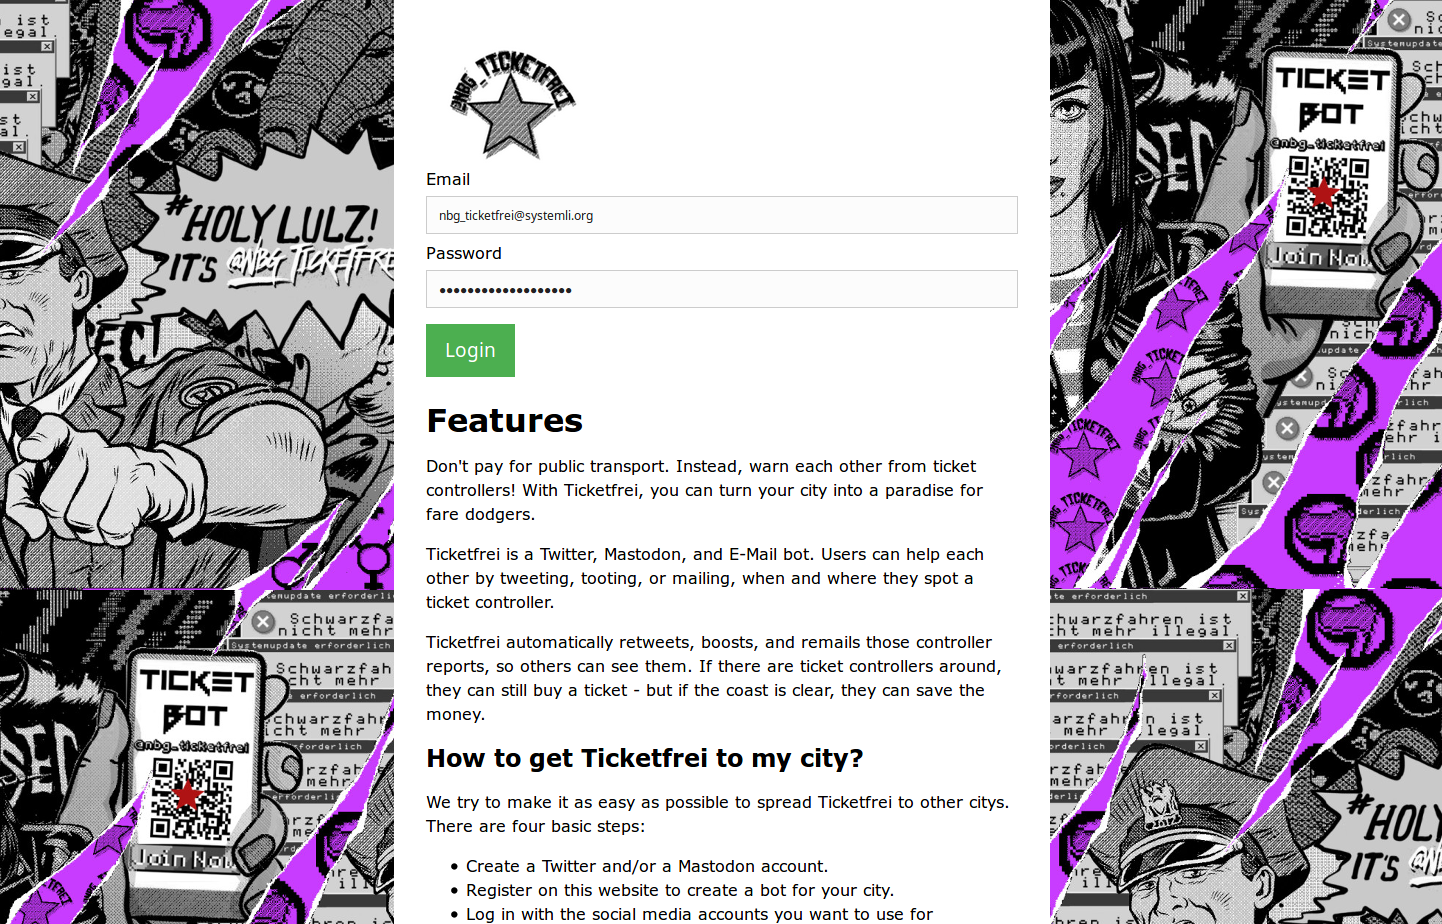
\includegraphics[width=\textwidth]{screenshots/Screenshot_2018-03-30_01-22-59.png}	
\end{frame}
\begin{frame}
	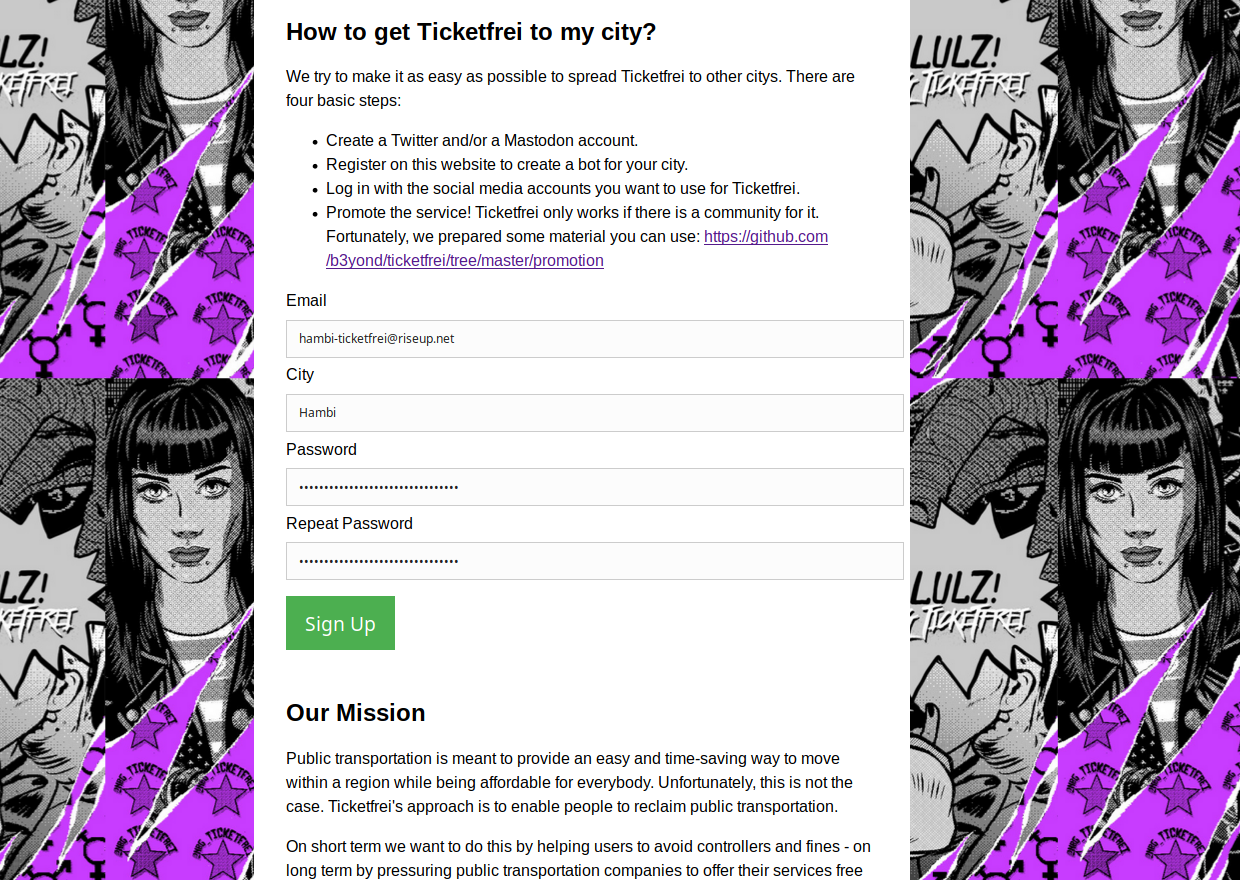
\includegraphics[width=\textwidth]{screenshots/Screenshot_2018-03-30_01-10-40.png}	
\end{frame}
\begin{frame}
	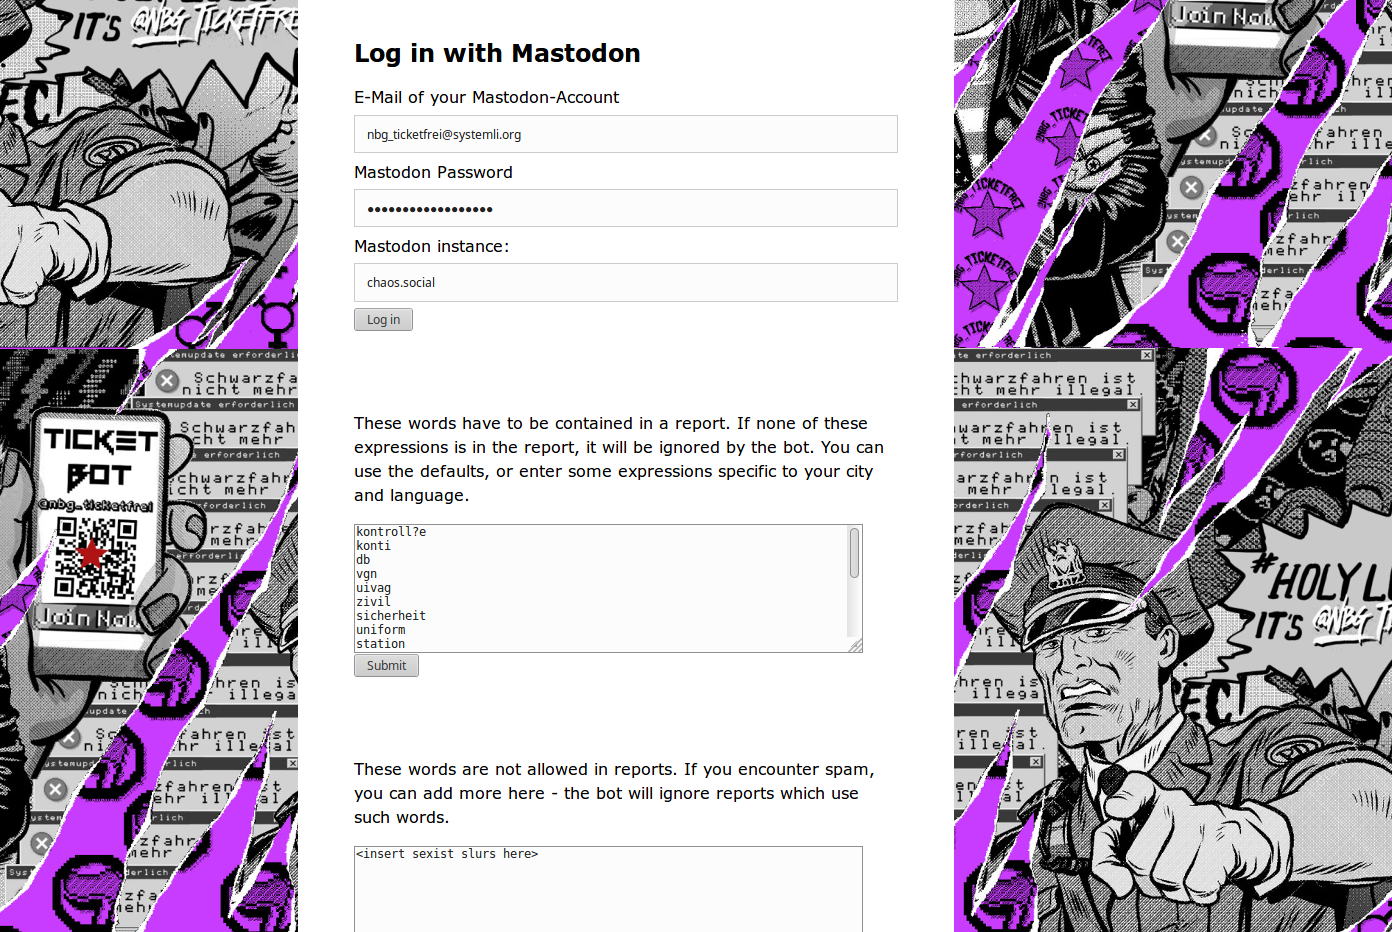
\includegraphics[width=\textwidth]{screenshots/Screenshot_2018-03-30_01-13-16.png}	
\end{frame}


\subsection{Step-by-Step}
\begin{frame}{The Ticketfrei Bot}{Step-by-Step}

\begin{itemize}
  \item Create an Account at https://ticketfrei.links-tech.org:
  \begin{itemize}
    \item E-Mail-Adress, City, Password
  \end{itemize}
  \item Add Social-Media accounts to your Ticketfrei account
  \item Change the text on https://ticketfrei.links-tech.org/city/Nürnberg
  \item Promote the use of the bot in your city
\end{itemize}

\end{frame}
\begin{frame}{The Ticketfrei Bot}{Step-by-Step}

\begin{block}{{Add Twitter}}
  \begin{itemize}
    \item Register a twitter account
    \item Click on "Login with Twitter" in the settings
    \item Log in to the twitter account of the bot
    \item Authorize the Ticketfrei app
  \end{itemize}
\end{block}

\end{frame}
\begin{frame}{The Ticketfrei Bot}{Step-by-Step}

\begin{block}{{Add Mastodon}}
  \begin{itemize}
    \item Register a mastodon account
    \item Enter the account's e-mail address, the password, and the mastodon server to the settings
    \item Click on "Log in"
  \end{itemize}
\end{block}

\end{frame}
\begin{frame}{The Ticketfrei Bot}{Step-by-Step}

\begin{block}{{Add Telegram}}
  \begin{itemize}
    \item Write to @botfather on Telegram to register a Telegram Bot
    \item Enter the API key which @botfather gives to you into the settings
    \item Click on "Login with Telegram"
  \end{itemize}
\end{block}

\end{frame}

\subsection{promotion}
\begin{frame}{The Ticketfrei Bot}{Promotion}

\begin{itemize}
  \item Leaflets in the local leftist scene, with more radical message
  \item Leaflets for the public, which explains goals and talks about the environment, but also explains the bot
  \item Example Leaflets are available in the GitHub-Repository at \url{https://github.com/b3yond/ticketfrei/tree/multi-deployment/promotion}
  \item<2-> Aktionsschwarzfahren is a good way to both spread leaflets and dodge the fare legally
  \item<3-> With enough public attention you can try to start a referendum or bring the topics to political parties for policy making
  \item<4-> Studies about the practicability and cost effectiveness of ticket-free public transport in your area are also useful
\end{itemize}

\end{frame}

%-------------------------------------------------------
\section{Sousveillance}
\subsection{Cybernetics and Surveillance}
\begin{frame}{Surveillance vs. Sousveillance}{1. Surveillance}
%-------------------------------------------------------

\begin{itemize}
  \item<1-> Cybernetics/Maxwell's Demon: if you know everything about the present, can you foretell the future?
  \begin{itemize}
    \item<2-> It does not matter if it really works
    \item<2-> Thesis: to prove that it does not work, I would need more data than the surveillers
  \end{itemize}
  \item<3-> Cybernetics comes from the greek word kybernetes: navigator, governor.
  \item<3-> It's about collecting as much data as possible, to link them to each other
  \item<3-> Keeping data secret ensures a knowledge edge against other parties
  \item<4-> It's only dangerous if surveillers can use violence
  \item<4-> You never know what data others have, or how it could be linked, so it's nearly impossible to protect yourself
\end{itemize}

\end{frame}

%-------------------------------------------------------
\subsection{Definition Sousveillance}
\begin{frame}{Surveillance vs. Sousveillance}{2. Sousveillance}
%-------------------------------------------------------

\begin{itemize}
  \item<1-> Definition Sousveillance:
  \begin{itemize}
    \item It's bottom-up surveillance -> the target is more powerful than you
    \item The results are published
    \item Contrast: sousveillance is neither espionage nor doxxing
  \end{itemize}
  \item<2-> Disciplining police and intelligence agencies can work
  \begin{itemize}
    \item<2-> It raises their costs for surveillance and power exercise
  \end{itemize}
  \item<2-> Keeping secrets is always harder than publication
\end{itemize}

\end{frame}

%-------------------------------------------------------
\subsection{Examples for Sousveillance}
\begin{frame}{Surveillance vs. Sousveillance}{Examples for Sousveillance}
%-------------------------------------------------------

\begin{itemize}
  \item<1-> Whistleblowers (ordered by coolness): Chelsea Manning, Edward Snowden, and WikiLeaks
  \item<1-> (Investigative-)Journalism: What are state \& corps actually doing?
  \begin{itemize}
    \item<2-> Panama Papers, Paradise Papers
  \end{itemize}
  \item<2-> Filming Demonstrations, Police controls, Police violence, etc.
  \begin{itemize}
    \item<2-> OccupyWallstreet had the biggest afflux, when videos about police violence surfaced
  \end{itemize}
  \item<3-> Ticketfrei: where are the ticket controllers, police cars, ...?
\end{itemize}

\end{frame}


%-------------------------------------------------------
\subsection{Conclusion}
\begin{frame}{Surveillance vs. Sousveillance}{Conclusion}
%-------------------------------------------------------

\text Surveillance won't vanish. Private property wants to be controlled, economic and political participation are not wanted. Surveillance enables this and emerges to completely new business models. Those business models are too powerful to be effectively combatted (see GDPR).

\text \break

\text So we have to defend ourselves, and sousveil the powerful. Sousveillance are an effective means against control society.

\end{frame}


{\1
\begin{frame}[plain,noframenumbering]
  \finalpage{Thank you for listening!}
\end{frame}}

\end{document}
